% This must be in the first 5 lines to tell arXiv to use pdfLaTeX, which is strongly recommended.
\pdfoutput=1
% In particular, the hyperref package requires pdfLaTeX in order to break URLs across lines.

\documentclass[11pt]{article}

% Remove the "guidelines" option to generate the final version.
\usepackage[guidelines]{nlpreport} % show guidelines
%\usepackage[]{nlpreport} % hide guidelines


% Standard package includes
\usepackage{times}
\usepackage{latexsym}
\usepackage{verbatim}

% For proper rendering and hyphenation of words containing Latin characters (including in bib files)
\usepackage[T1]{fontenc}
% For Vietnamese characters
% \usepackage[T5]{fontenc}
% See https://www.latex-project.org/help/documentation/encguide.pdf for other character sets

% This assumes your files are encoded as UTF8
\usepackage[utf8]{inputenc}

% This is not strictly necessary, and may be commented out,
% but it will improve the layout of the manuscript,
% and will typically save some space.
\usepackage{microtype}
\usepackage{graphicx}
\usepackage{hyperref}
\usepackage{amsmath}
\usepackage{mathtools}
\usepackage{multirow}
\usepackage{listings}
\usepackage{xcolor}
\usepackage{booktabs} % for tables

% THE pdfinfo Title AND Author ARE NOT NECESSARY, THEY ARE METADATA FOR THE FINAL PDF FILE
\hypersetup{pdfinfo={
Title={Assignment 1: Part-Of-Speech Tagging},
Author={Jane Smith \& John Doe}
}}
%\setcounter{secnumdepth}{0}  
 \begin{document}
%
\title{Assignment 1: Part-Of-Speech Tagging on the Penn Treebank Tagset}

\author{Mattia Maranzana,
Antonios Pantelis,
\and
Nalin Sharma\\
Master's Degree in Artificial Intelligence, University of Bologna\\
\{mattia.maranzana, antonios.pantelis, nalin.sharma\}@studio.unibo.it
}
\maketitle

\begin{comment}
\attention{DO NOT MODIFY THIS TEMPLATE - EXCEPT, OF COURSE FOR TITLE, SUBTITLE AND AUTHORS.\\ IN THE FINAL VERSION, IN THE \LaTeX\ SOURCE REMOVE THE \texttt{guidelines} OPTION FROM  \texttt{$\backslash$usepackage[guidelines]\{nlpreport\}}.
}
\end{comment}

\begin{abstract}
%\begin{quote}
In this project we are called to address the classification task of Part of Speech (POS) Tagging on the pre-tagged Penn Treebank Tagset. Our goal is to elevate accuracy, leveraging the text pre-processing and NLP model development techniques that we explored in the course and during Tutorials 1 and 2.
%\end{quote}
\end{abstract}

\begin{comment}
\attention{\textcolor{red}{NOTICE: THIS REPORT'S LENGTH MUST RESPECT THE FOLLOWING PAGE LIMITS: \begin{itemize}
    \item ASSIGNMENT: \textbf{2 PAGES} 
    \item NLP PROJECT OR PROJECT WORK: \textbf{8 PAGES}
    \item COMBINED NLP PROJECT + PW: \textbf{12 PAGES}
\end{itemize}  PLUS LINKS, REFERENCES AND APPENDICES.\\ 
THIS MEANS THAT YOU CANNOT FILL ALL SECTIONS TO MAXIMUM LENGTH. IT ALSO MEANS THAT, QUITE POSSIBLY, YOU WILL HAVE TO LEAVE OUT OF THE REPORT PART OF THE WORK YOU HAVE DONE OR OBSERVATIONS YOU HAVE. THIS IS NORMAL: THE REPORT SHOULD EMPHASIZE WHAT IS MOST SIGNIFICANT, NOTEWORTHY, AND REFER TO THE NOTEBOOK FOR ANYTHING ELSE.\\ 
FOR ANY OTHER ASPECT OF YOUR WORK THAT YOU WOULD LIKE TO EMPHASIZE BUT CANNOT EXPLAIN HERE FOR LACK OF SPACE, FEEL FREE TO ADD COMMENTS IN THE NOTEBOOK.\\ 
INTERESTING TEXT EXAMPLES THAT EXCEED THE MAXIMUM LENGTH OF THE REPORT CAN BE PLACED IN A DEDICATED APPENDIX AFTER THE REFERENCES.}}
\end{comment}

\section{Introduction}

As we mentioned previously, we are addressing the supervised learning task of POS tagging on the Penn Treebank dataset. Let us give a brief summary of our approach.

We encoded the Tagset into a \texttt{pandas} dataframes, namely \texttt{df} split by sentences. Then we split \texttt{df} into training, validation, and test sets, adding an additional "split" column to identify each piece of data with its corresponding dataset.

Then, we performed basic data inspection, visualizations, and text pre-processing, as detailed in section "\nameref{sec:data}."

Furthermore, we built the vocabulary of the corpus, along with \texttt{idx\_to\_word} and \texttt{word\_to\_idx} maps, and conducted tokenization.

Next up, we built the embedding matrix and calculated Out of Vocabulary (OOV) words percentage.

Subsequently, we performed some data preparation that included One-Hot Encoding, and size verification.

Later on, we created a variable, \texttt{punctuation\_indices}, to store punctuation indices for later exclusion during metric evaluation, developed a macro multi-class $F_1$ score metric and proceeded to create the three models.

Finally, after training our models, we conducted basic error analysis by identifying misclassified tags and their corresponding words to explore potential correlations.


\section{System description}
\label{sec:system}

For the creation of our models, we used the \texttt{Keras}\footnote{This was precisey the reason why we had to define the metric $F_1$ ourselves, since the already defined one of \texttt{scikit-learn} is incompatible with \texttt{Tensorflow}.} library of \texttt{Tensorflow}. As instructed, we developed three models, whose architectures can be seen in Figure \ref{fig:Models}.

We worked with GloVe embeddings and after calculating the OOV words percentage we proceeded as follows: For the validation and test sets, we addressed OOV words by replacing them with token "UNK". The subsequent creation of an embedding matrix involved using GloVe embeddings for known words, zero vectors for "UNK", and random vectors for remaining OOV words. Moreover, padding was applied at the beginning of each sequence, and sentences exceeding a length of 600 were truncated.

\begin{figure*}
    \begin{minipage}{.3\textwidth}
      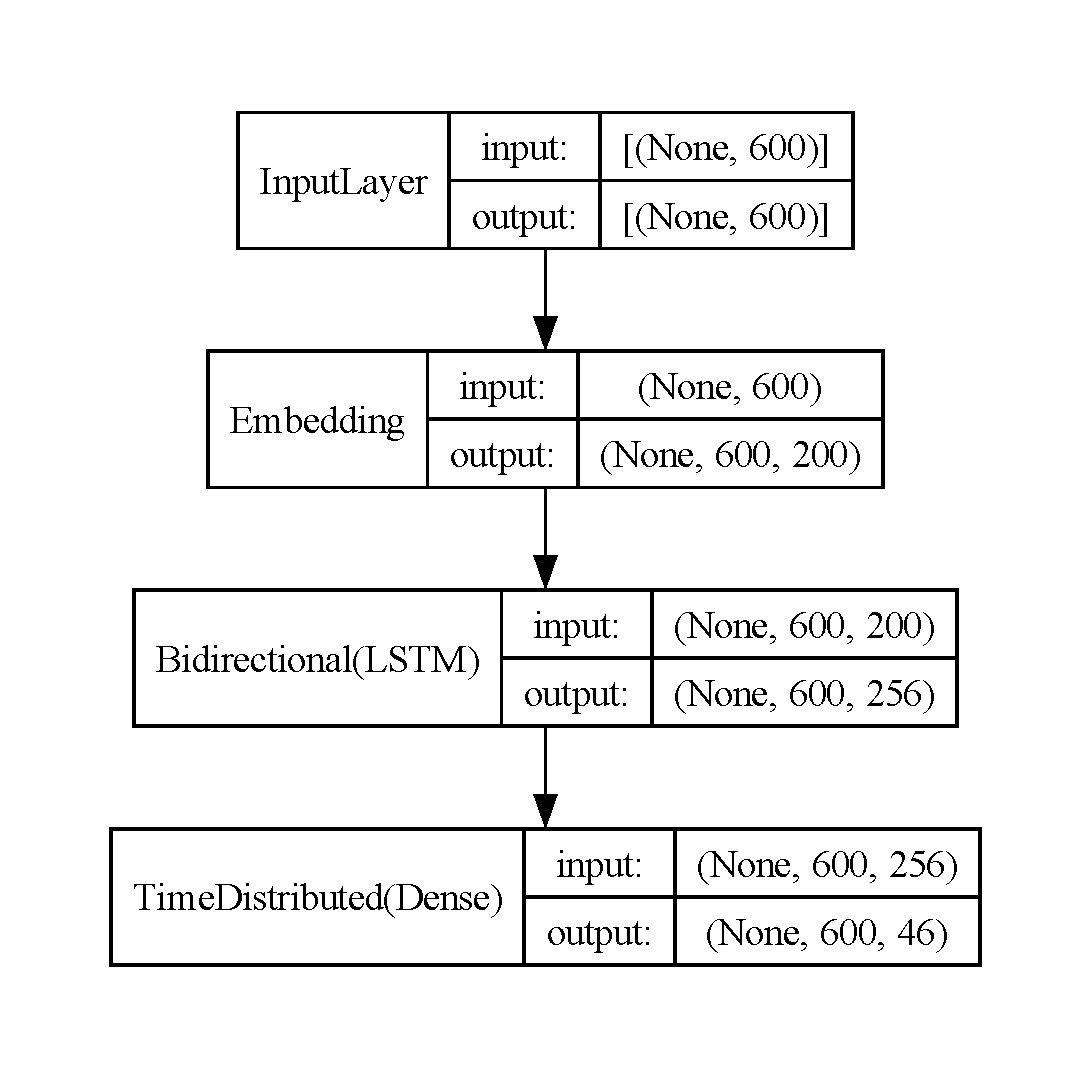
\includegraphics[width=\linewidth]{baseline_model.pdf}
      %\caption{Baseline Model}
      %\label{fig:baseline}
    \end{minipage} \quad
    \begin{minipage}{.3\textwidth}
      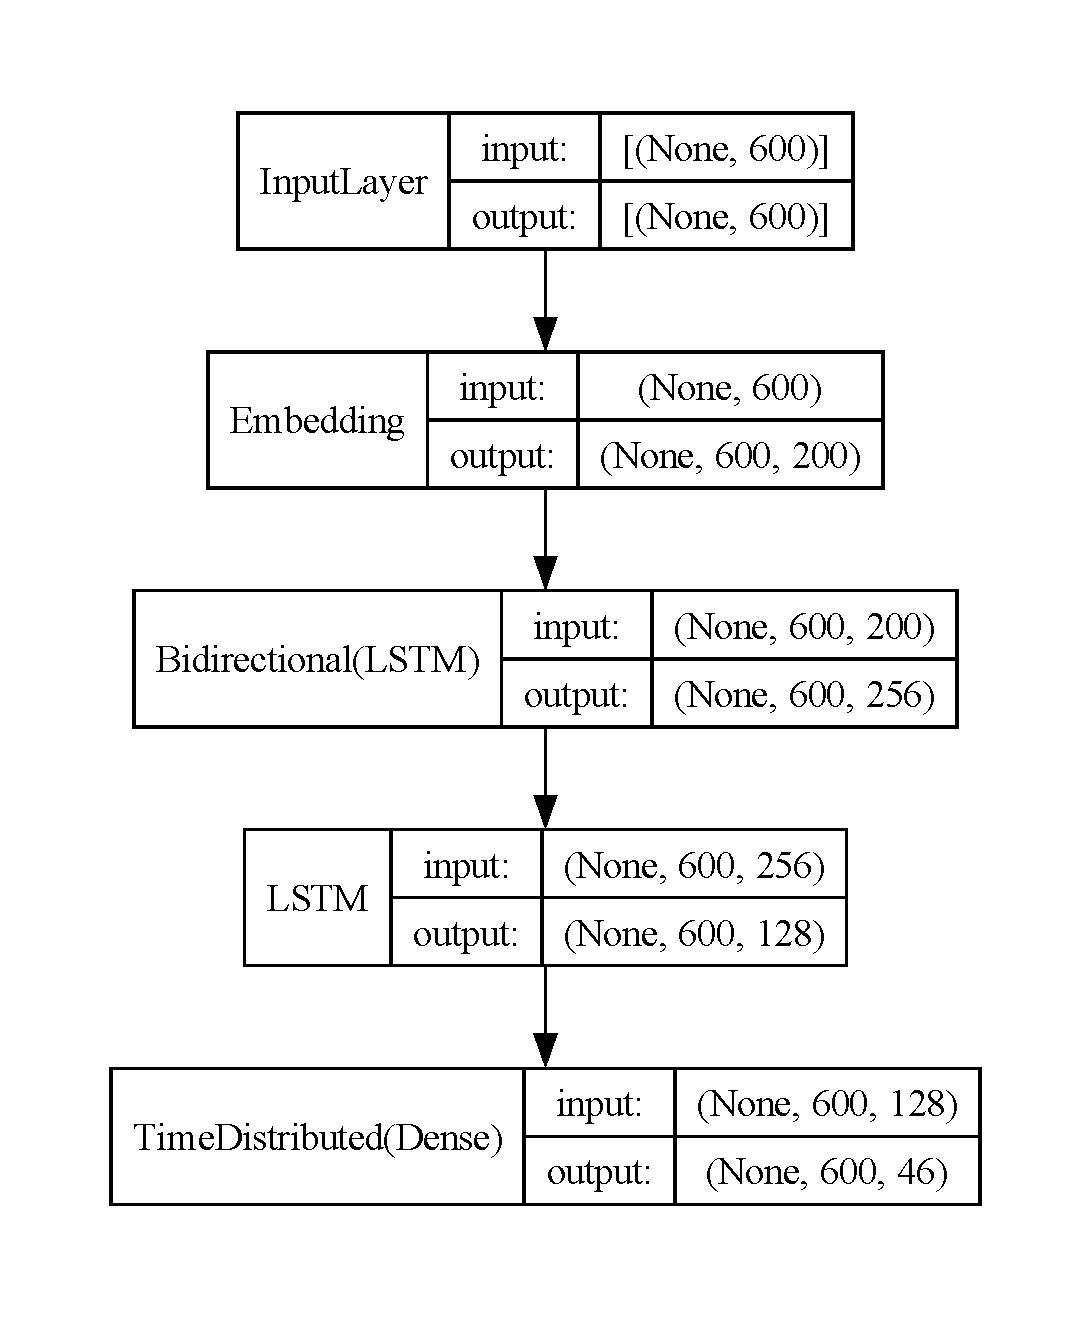
\includegraphics[width=\linewidth]{model_1.pdf}
      %\caption{Model 1}
      %\label{fig:model1}
    \end{minipage} \quad
    \begin{minipage}{.3\textwidth}
      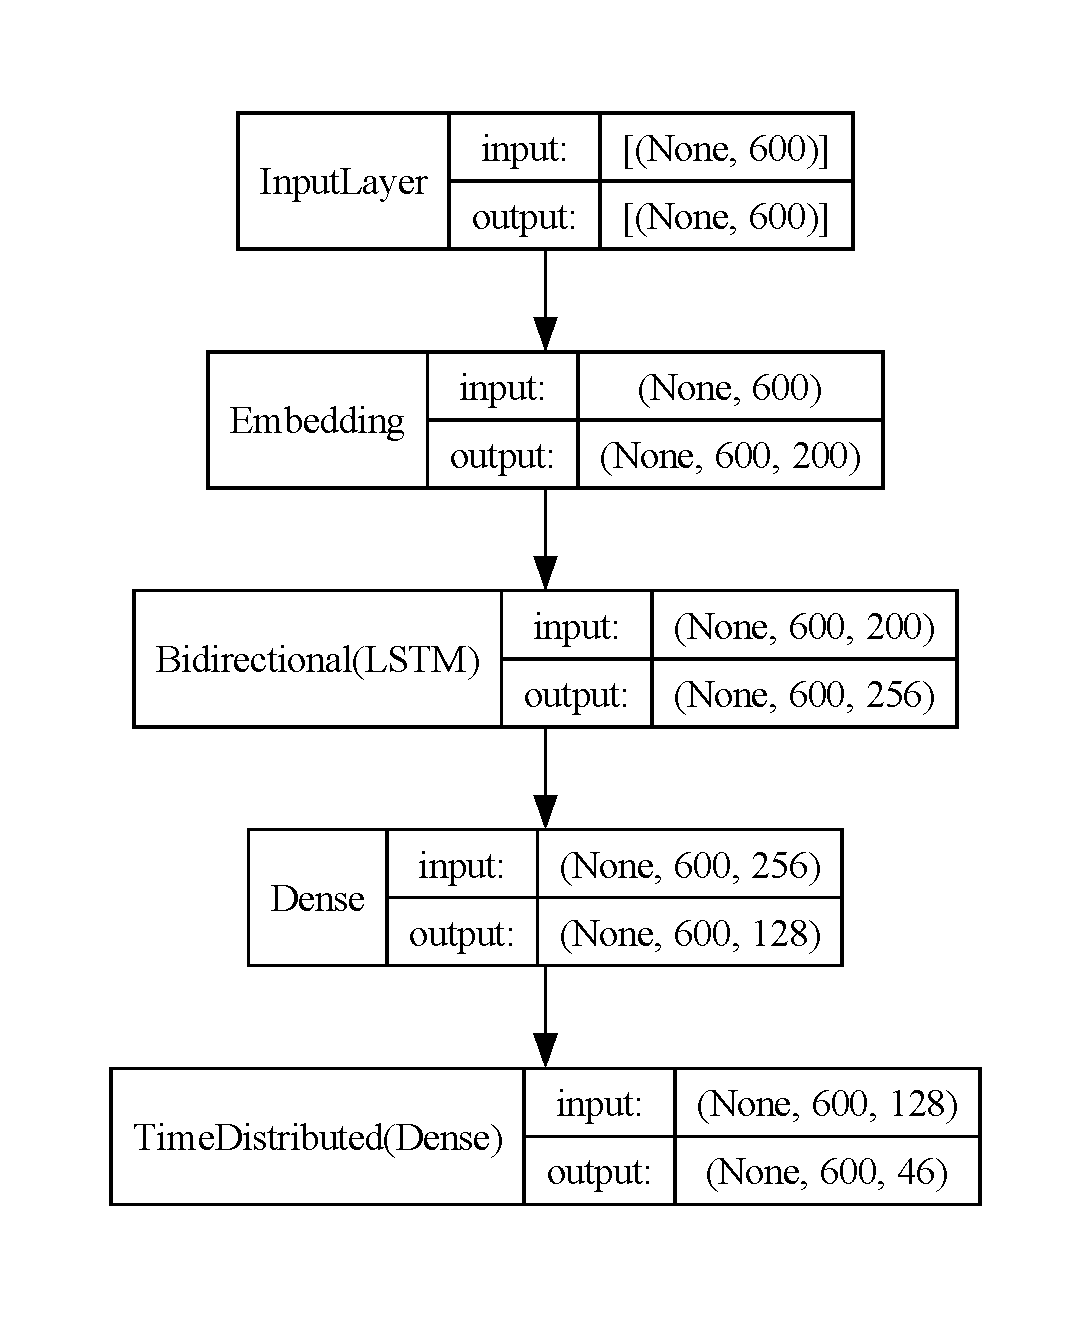
\includegraphics[width=\linewidth]{model_2.pdf}
      %\caption{Model 2}
      %\label{fig:model2}
    \end{minipage}
    \caption{Architectures of \texttt{baseline\_model} (left), \texttt{model\_1} (center), and \texttt{model\_2} (right).}
    \label{fig:Models}
\end{figure*}

\section{Data}
\label{sec:data}
As far as data inspection goes, we calculated the distribution of individual words in sentences and the distribution of POS tags and plotted the 20 \emph{most}\footnote{Most of the \emph{most frequent} words included punctuation and stop words.} and \emph{least frequent}\footnote{Some of the \emph{least frequent} words included numbers and names.} words. 

Furthermore, we created a dictionary for the POS labels and performed some minimal text pre-processing on the corpus. In particular, we chose to simply make every word in the corpus lower case, since we could not delete or modify any tokens. This helped greatly with the OOV words percentage. In particular, we obtained $4.98\%$ after lower-casing, while before we had obtained approximately $20\%$. This made the OOV percentage negligible and thus we decided that no further handling of the OOV words was required.

Moreover, we also plotted two box plots showing the distribution of sentences' lengths. This helped us make an informed decision about the padding. Since the beginning of the project we had two ideas in mind: either truncate sequences at a fixed padding length with the risk of losing some information, or trying to divide each file in sub-sentences of fixed length and pad them accordingly as not to lose any information at all. However, from the two box plots in question, it was clear that the more convenient one is that of truncating each sentence at length equal to 600. With this choice, we lose only a negligible amount of information out of only one sentence whose length is as one can see from both box plots around twice the padding length.

\section{Experimental setup and results}

Hyperparameters for the neural POS tagger were tuned using Gridsearch across the following values:



\begin{table}[ht]
\centering
\begin{tabular}{ll}
\toprule
\textbf{Hyperparameter} & \textbf{Values} \\
\midrule
Embedding Dimensions & 50, 100, 200, 300 \\
Batch Sizes & 32, 64, 128 \\
LSTM Sizes & 32, 64, 128 \\
Learning Rates & 0.001, 0.01, 0.1 \\
Trainable embeddings & True, False \\
\bottomrule
\end{tabular}
\end{table}

After the Gridsearch, we obtained the best-performing hyperparameters as follows: 200 for the embedding dimension, 128 for batch and LSTM size, 0.01 for learning rate and True for trainability of the embedding layer (Results in Appendix A below).

Models were evaluated based on their macro F1 score, reflecting performance across all classes.


% can throw in the appendix if it doesn't fit here 

\section{Discussion}
\label{sec:discussion}

The baseline BiLSTM model coupled with a dense layer, trained on GloVe embeddings produces appreciable performance with respect to models 1 and 2 (Results in Appendix A below). Model 1 shows a noticeable drop in macro f1 score, hinting that the additional complexity does not translate to better representation for this task, potentially interfering with the effective features already provided with GloVe. Model 2 improves on this slightly, suggesting that the layer provides nuanced classification by leveraging its non-linear transformations. However, both models are evidently overfitting with their added complexity.
\newline
Regarding error analysis, our most frequently misclassified words were slangs/specialised vocabulary that were in our OOV set. To improve this, we could use Byte Pair Encoding, to allow the model to understand embeddings for unknown words based on known subword units. We can also fine-tune the GloVe embeddings on a domain-specific corpus. 



\section{Conclusion}
\label{sec:conclusion}
Contrary to our expectations, the baseline model remained sufficiently complex for this task, achieving competitive macro f1 scores around 0.7 across all 3 seeds. This speaks to the richness of the GloVe embeddings, and the effectiveness of transfer learning and fine-tuning routine in the defined model.

Nevertheless, static GloVe embeddings do not capture the full contextual boundaries of the data. Using models such as BERT or GPT, we can leverage more context-aware embeddings. The model also misrepresents some compound words, thus better handling of the linguistic variability in the corpora is required for future works. 


\section{Appendix A}
\label{sec:results}
\begin{table}[ht]
\centering
\begin{tabular}{|c|c|c|c|}
\hline
\textbf{Seed} & \textbf{Model} & \textbf{Loss} & \textbf{Macro F1 Score} \\ \hline
\multirow{3}{*}{47} & Baseline & 0.69 & 0.74 \\
 & Model 1 & 0.0198 & 0.69 \\
 & Model 2 & 0.01 & 0.72 \\ \hline
\multirow{3}{*}{652} & Baseline & 0.014 & 0.68 \\
 & Model 1 & 0.01 & 0.61 \\
 & Model 2 & 0.01 & 0.68 \\ \hline
\multirow{3}{*}{72} & Baseline & 0.01 & 0.68 \\
 & Model 1 & 0.01 & 0.63 \\
 & Model 2 & 0.01 & 0.67 \\ \hline
\end{tabular}
\caption{Model Performance with Different Seeds}
\label{table:results}
\end{table}

\end{document}

